\section{Evaluation}

We evaluate Agent-Sentinel on the regenerated 200-scenario benchmark and on the small real-agent case study described elsewhere in the paper. The main benchmark is the primary source for the baseline comparison because it exercises both policy-deny behavior and robustness behavior under a shared execution harness.

\subsection{Workload Categories}

The benchmark is divided into three layers. Safe categories contain benign and trace-stress tasks that should be allowed. Security-deny categories contain malicious and policy-blocked tasks that should be denied before tool execution. Robustness categories contain malformed-payload and plugin-failure tasks that should not be counted as successful security blocks, but should still be reported because they expose execution-path fragility and plugin-isolation behavior.

\subsection{Baseline Comparison}

Table~\ref{tab:evaluation_results} reports the main benchmark results. The systems compared are No Protection, Static Allowlist, Argument Allowlist, Validator Only, Progent-style, No Audit, and full Agent-Sentinel.

\begin{table*}[t]
\centering
\small
\setlength{\tabcolsep}{7pt}
\caption{Baseline comparison across the Agent-Sentinel evaluation suite. The table reports attack blocking effectiveness, safe-action allowance, and runtime latency across different defense configurations.}
\label{tab:evaluation_results}
\begin{tabular}{lrrrr}
\toprule
System & Unsafe Actions Blocked (\%) & Safe Actions Allowed (\%) & Median Latency (ms) & p95 Latency (ms) \\
\midrule
No Protection & 0.00 & 100.00 & 0.02 & 0.10 \\
Static Allowlist & 50.60 & 100.00 & 0.02 & 0.09 \\
Argument Allowlist & 83.13 & 100.00 & 0.06 & 0.24 \\
Validator Only & 72.29 & 100.00 & 0.05 & 0.14 \\
No Audit & 100.00 & 100.00 & 0.07 & 0.30 \\
Progent-style & 67.47 & 100.00 & 0.05 & 0.18 \\
\textbf{Agent-Sentinel} & \textbf{100.00} & \textbf{100.00} & 0.24 & 0.60 \\
\bottomrule
\end{tabular}
\end{table*}


All systems preserve 100.0\% of safe actions on the current workload. The primary distinction is therefore in how much of the security-deny slice each system blocks, and whether that improvement comes from richer runtime mediation or only from narrower tool-name rules.

\subsection{Live OpenAI Evaluation}

Table~\ref{tab:live_eval_summary} reports the aggregate count-based view of the five-run OpenAI-backed live evaluation. Across 200 executions, the model preserved all benign tasks and handled all robustness tasks without execution errors, preserving the expected robustness outcomes across runs. All 100 attack executions were denied overall, but only 65 were explicitly blocked by Agent-Sentinel; the remaining 35 were model-side no-tool refusals.

\begin{table}[t]
\centering
\small
\renewcommand{\arraystretch}{1.12}
\setlength{\tabcolsep}{6pt}
\caption{Live OpenAI-backed evaluation summary for the 80x5 benchmark.}
\label{tab:live_eval_summary}
\begin{tabular}{@{}p{0.74\linewidth}r@{}}
\toprule
Metric & Value \\
\midrule
Total live executions & 400 \\
Benign tasks & 150 \\
Attack tasks & 200 \\
Robustness tasks & 50 \\
\addlinespace
Benign preservation rate & 100.0\% \\
Attack prevention rate & 100.0\% \\
Explicit Sentinel block rate on attacks & 65.0\% \\
Model no-tool denials on attacks & 70 \\
\addlinespace
Median latency & 2469.3 ms \\
P95 latency & 4977.3 ms \\
Max latency & 9404.5 ms \\
\bottomrule
\end{tabular}
\end{table}


Table~\ref{tab:live_eval_main_results} distills the paper-facing claims, while Figure~\ref{fig:live_eval_outcomes} visualizes the outcome composition by task class.

\begin{table}[t]
\centering
\small
\renewcommand{\arraystretch}{1.12}
\setlength{\tabcolsep}{6pt}
\caption{Main results for the 80x5 live evaluation.}
\label{tab:live_eval_main_results}
\begin{tabular}{@{}p{0.71\linewidth}r@{}}
\toprule
Metric & Result \\
\midrule
Total live executions & 400 \\
Benign tasks & 150 \\
Attack tasks & 200 \\
Robustness tasks & 50 \\
\addlinespace
Benign preservation rate & 100.0\% \\
Attack prevention rate & 100.0\% \\
Explicit Sentinel block rate on attacks & 65.0\% \\
Model-only denials & 70 \\
\bottomrule
\end{tabular}
\end{table}

\begin{figure}[t]
\centering
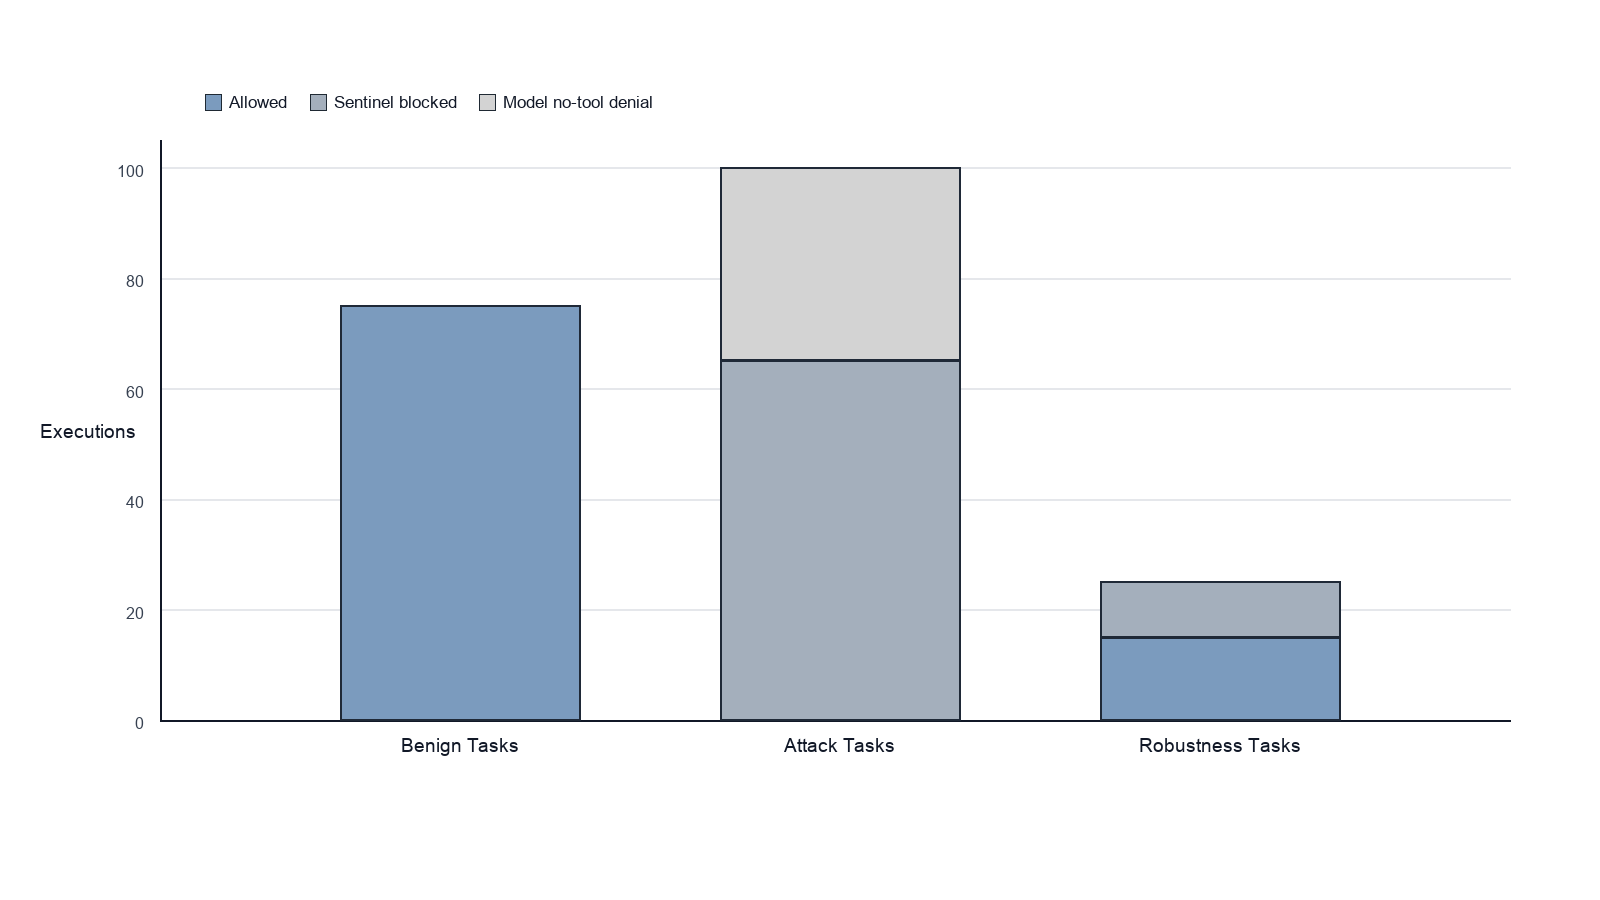
\includegraphics[width=\linewidth]{figures/fig_live_eval_outcomes.png}
\caption{Live evaluation outcomes across benign, attack, and robustness tasks.}
\label{fig:live_eval_outcomes}
\end{figure}


Figure~\ref{fig:live_eval_latency_boxplot} summarizes the latency distribution across benign, attack, and robustness tasks. Table~\ref{tab:live_eval_stability} confirms that the results are stable across the five runs.

\begin{figure}[t]
\centering
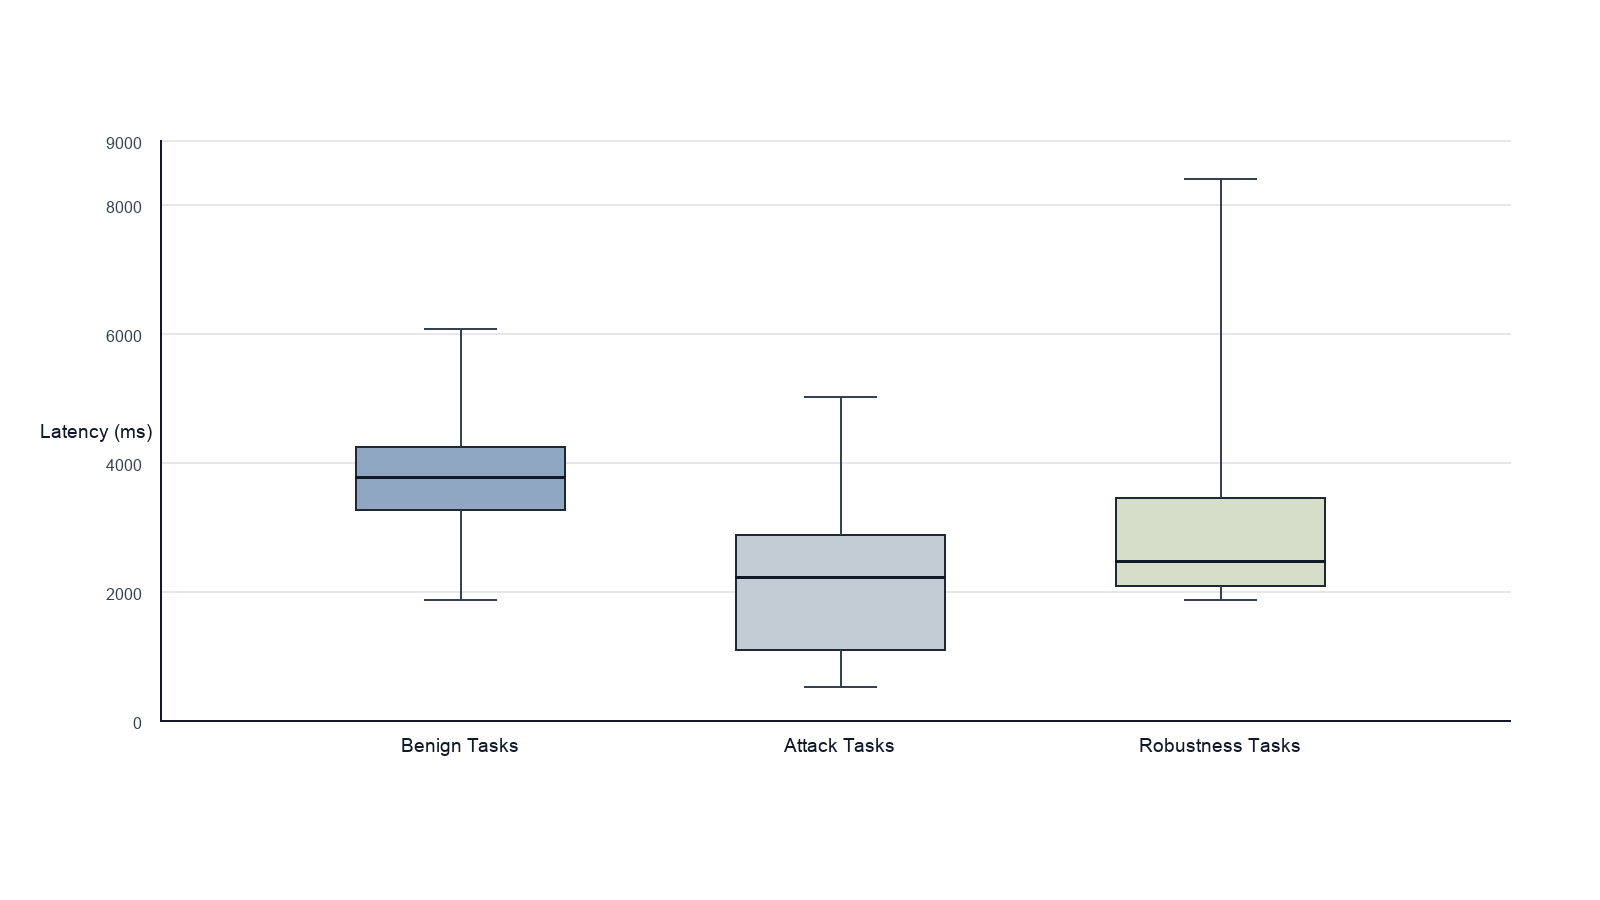
\includegraphics[width=\linewidth]{figures/fig_live_eval_latency_boxplot.png}
\caption{Latency distribution across the 80x5 live evaluation.}
\label{fig:live_eval_latency_boxplot}
\end{figure}

\begin{table}[t]
\centering
\small
\renewcommand{\arraystretch}{1.12}
\setlength{\tabcolsep}{6pt}
\caption{Run-to-run stability of the live evaluation.}
\label{tab:live_eval_stability}
\begin{tabular}{@{}p{0.67\linewidth}r@{}}
\toprule
Metric & Mean $\pm$ Std \\
\midrule
Benign preservation rate & 100.0\% $\pm$ 0.0\% \\
Attack prevention rate & 100.0\% $\pm$ 0.0\% \\
Robustness handled rate & 100.0\% $\pm$ 0.0\% \\
Explicit Sentinel block rate on attacks & 65.0\% $\pm$ 3.5\% \\
Model self-denial rate on attacks & 35.0\% $\pm$ 3.5\% \\
Median latency & 2750.96 $\pm$ 218.55 ms \\
P95 latency & 4898.59 $\pm$ 642.75 ms \\
\bottomrule
\end{tabular}
\end{table}


Table~\ref{tab:live_attack_breakdown} provides a compact category-level breakdown of the attack subset.

\begin{table}[t]
\centering
\small
\renewcommand{\arraystretch}{1.1}
\setlength{\tabcolsep}{6pt}
\caption{Attack-category breakdown of the 80x5 live evaluation.}
\label{tab:live_attack_breakdown}
\begin{tabular}{@{}lrrrr@{}}
\toprule
Category & Total & Deny & Blocked & Blocked Rate (\%) \\
\midrule
\texttt{absolute-path} & 35 & 35 & 13 & 37.1 \\
\texttt{private-file} & 20 & 20 & 20 & 100.0 \\
\texttt{traversal} & 20 & 20 & 5 & 25.0 \\
\texttt{cross-tool} & 15 & 15 & 15 & 100.0 \\
\texttt{domain-denied} & 15 & 15 & 10 & 66.7 \\
\texttt{exfiltration} & 15 & 15 & 10 & 66.7 \\
\texttt{metadata} & 15 & 15 & 15 & 100.0 \\
\texttt{prompt-injection} & 15 & 15 & 6 & 40.0 \\
\texttt{path-normalization} & 10 & 10 & 10 & 100.0 \\
\texttt{private-write} & 10 & 10 & 5 & 50.0 \\
\texttt{ssh-key} & 10 & 10 & 10 & 100.0 \\
\texttt{mixed-case-domain} & 5 & 5 & 5 & 100.0 \\
\texttt{obfuscated-path} & 5 & 5 & 1 & 20.0 \\
\texttt{obfuscated-url} & 5 & 5 & 5 & 100.0 \\
\texttt{query-exfiltration} & 5 & 5 & 0 & 0.0 \\
\bottomrule
\end{tabular}
\end{table}

